\documentclass[11pt]{article}
\usepackage[T1]{fontenc}
\usepackage[margin=1in]{geometry}
\usepackage{amsmath,amssymb}
\usepackage{graphicx}
\usepackage{booktabs}
\usepackage{longtable}
\usepackage{array}
\usepackage{xcolor}
\usepackage{tikz}
\usetikzlibrary{arrows.meta,positioning,fit,backgrounds,calc,decorations.pathreplacing}
\usepackage[colorlinks=true,linkcolor=blue!60!black,urlcolor=blue!60!black,
            citecolor=blue!60!black]{hyperref}
\usepackage[htt]{hyphenat}
\usepackage{microtype}
\emergencystretch=3em
\usepackage{listings}
\lstset{basicstyle=\ttfamily\footnotesize, backgroundcolor=\color{gray!8},
        frame=single, rulecolor=\color{gray!40}, breaklines=true,
        columns=fullflexible, keepspaces=true, showstringspaces=false}

\newcommand{\code}[1]{\texttt{#1}}
\newcommand{\file}[1]{\texttt{\small #1}}
\newcommand{\fn}[1]{\texttt{\small #1}}
\newcommand{\Om}{\Omega_0}
\newcommand{\qom}{q\Om}

\title{Orbital Advection Across Azimuthal Level Jumps\\
       in the AthenaK Shearing Box\\[0.4em]
       \large \textsc{Implementation Document}}
\author{\code{athenak-multigrid} tree, branch \code{fargo-amr}\\
        \small parent commit \code{d3edb948} (branch \code{dust-multigrid})}
\date{October 28, 2026}

\begin{document}
\maketitle

\begin{abstract}
\noindent
With orbital advection (FARGO) on, AthenaK's shearing box could be refined only in
complete azimuthal rings: every $x_2$ neighbor of a MeshBlock had to be at its own level.
For clump-following adaptive refinement that is the dominant cost --- a fragment in the
$64H$ SC14 box refines a $64H$-long ring at every level. This document describes how the
cell-centered orbital remap was extended so that an $x_2$ neighbor may be one level
coarser or finer. Each block still remaps on its own grid; the neighbor's rows are
restricted (from a finer neighbor) or prolongated (from a coarser one) to the block's
resolution before the remap. The remap is rewritten in flux form, and an orbital-advection
flux correction makes it exactly conservative across the level jump. A timestep limit
keeps the shift within the immediate neighbor. The ring policy becomes an option. Uniform
and ring-refined runs are bit-identical to the parent code. For MHD (branch
\code{fargo-amr-mhd}) the same holds: the face-field remap brings the neighbour's $B_1$,
$B_3$ rows to each block's resolution, and its effective EMFs are corrected at level jumps
like the stage EMFs, which keeps the two copies of every face shared by a fine and a coarse
block equal.
The tests are in the companion \file{fargo\_amr\_validation.pdf}.
\end{abstract}

\tableofcontents
\newpage

%=========================================================================================
\section{Scope and how to read this}
\label{sec:scope}

This document describes mechanisms --- data layout, index maps, call sites, guards ---
not results; those are in \file{fargo\_amr\_validation.pdf}. It builds on the shearing-box
refinement work documented in \file{multigrid\_sb\_implementation.pdf} (Phase 0 there:
the refinement policy, per-level orbital advection, the non-FARGO mode, AMR rebuilds of
the shear state). That document now carries short pointers here where its statements
about the ring policy are out of date.

\subsection{Files touched}
\begin{center}
\small
\begin{tabular}{@{}>{\raggedright\arraybackslash}p{5.2cm}p{9.2cm}@{}}
\toprule
File & Change \\
\midrule
\file{src/shearing\_box/orbital\_advection\_cc.cpp} & Rewritten: pack (same,
restricted, coarse-box messages), unpack with prolongation, remap fluxes $G$ at the block
faces, \fn{SendFluxCC}, \fn{RecvAndCorrectFluxCC}, \fn{RowsAvailable},
\fn{MaxTimeStep} \\
\file{src/shearing\_box/orbital\_advection.hpp} & \fn{OrbitalAdvectionCC} buffers,
sizes, MPI requests; virtual \fn{InitRecv}/\fn{ClearRecv}/\fn{ClearSend} \\
\file{src/shearing\_box/orbital\_advection\_tasks.cpp} & CC overrides of the three
MPI functions (per-sub-face requests, flux receives) \\
\file{src/hydro/hydro\{.hpp,\_tasks.cpp\}} & Tasks \fn{SendFlx\_OA}, \fn{RecvFlx\_OA} \\
\file{src/dust/dust\{.hpp,\_tasks.cpp\}} & Same two tasks in the dust module's copy of
the hydro task tail \\
\file{src/mesh/mesh.cpp} & Orbital-advection timestep limit in \fn{Mesh::NewTimeStep};
policy warning text \\
\file{src/mesh/build\_tree.cpp} & Ring check (I2) only with \code{oa\_annular} \\
\file{src/mesh/mesh\_refinement.\{cpp,hpp\}} & Ring-wise flag sync only with
\code{oa\_annular} \\
\file{src/hydro/hydro.cpp}, \file{src/mhd/mhd.cpp} & Comments \\
\file{src/pgen/tests/shwave.cpp} & Optional $x_2$ window for the moving-ring criterion
(a moving box) \\
\midrule
\multicolumn{2}{@{}l}{\textbf{MHD on rings (branch \code{fargo-amr-mhd})}}\\
\file{src/shearing\_box/orbital\_advection\_fc.cpp} & EMF correction of the face-field
remap (\fn{SendEMF\_OA}, \fn{RecvEMFAndUpdateB\_OA}, \fn{UpdateB}); buffer depth
\code{nrowb} $\le n_{x2}$; EMF arrays sized for AMR \\
\file{src/shearing\_box/orbital\_advection\{.hpp,\_tasks.cpp\}} & FC overrides of
\fn{InitRecv}/\fn{ClearRecv}/\fn{ClearSend} \\
\file{src/mhd/mhd\{.cpp,.hpp,\_tasks.cpp\}} & Guard relaxed to rings; tasks
\fn{SendE\_OA}, \fn{RecvE\_OA}, \fn{SendFlx\_OA}, \fn{RecvFlx\_OA} \\
\file{src/pgen/tests/swing.cpp} & History columns \code{bmis}, \code{bnrm}: shared-face
consistency; optional $x_2$ window of the moving-ring criterion; Jeans-length
criterion \fn{SwingJeansRefine} (\S\ref{sec:jeanscrit}) \\
\file{src/shearing\_box/orbital\_advection\_fc.cpp} (second step) & $B_1$, $B_3$ rows across
$x_2$ level jumps: per-sub-face buffers, area-averaged and interpolated messages \\
\bottomrule
\end{tabular}
\end{center}

%=========================================================================================
\section{Background}
\label{sec:background}

\subsection{Orbital advection in AthenaK}
In the shearing box the background flow is $v_y = -\qom x$. With orbital advection the
state carries only the deviation from it, and the background transport is applied as a
separate step: at the end of each time step (last RK stage, after the source terms) every
cell is shifted in $x_2$ by
\begin{equation}
  \Delta y = -\qom\, x_1\, \Delta t = (J + \epsilon)\,\Delta x_2,
  \qquad J = \operatorname{trunc}(\Delta y/\Delta x_2),\quad |\epsilon| < 1,
\end{equation}
per $x_2$ column (fixed $x_1$, $x_3$). The integer part $J$ is a copy, the fractional part a
conservative remap with upwind ``fluxes'' $F$ from a PLM or PPM reconstruction
(\file{remap\_fluxes.hpp}):
\begin{equation}
  a^{\rm new}_j = a_{j-J} - \left(F_{j-J+1/2} - F_{j-J-1/2}\right).
  \label{eq:remap}
\end{equation}
\fn{PackAndSendCC} sends the rows next to each $x_2$ face to the neighbor;
\fn{RecvAndUnpackCC} builds an extended column (own cells plus neighbor rows on both
sides) in team scratch memory and applies Eq.~\eqref{eq:remap}. The tasks
\fn{SendU\_OA}/\fn{RecvU\_OA} sit between the source terms and \fn{RestrictU} of the last
stage, so the shifted state then goes through the normal boundary exchange.

\subsection{The annular policy and what it cost}
The old pack used the same indices on both sides of a face (``neighbor must always be at
same level'') and read only neighbor slots 8 and 12, the first sub-face of each $x_2$ face.
A coarser neighbor, which sits in sub-face slot $9$--$11$ or $13$--$15$, was not even
read. Invariant I2 (complete $x_2$ rings at every level, with a ring-wise OR/AND of AMR
flags) kept every $x_2$ neighbor at the same level. In the SC14 clump-following AMR
runs ($64H\times64H\times16H$, $8^3$ blocks) a fragment's refinement therefore covered the
whole $64H$ azimuth at every level, reaching $\sim$28\,000 blocks at $\beta = 4$ and
70--100\,000 in the first $\beta = 3$ attempt.

\subsection{Prior art: Athena++}
Athena++'s orbital advection (T.~Ono) supports refinement. Each block remaps on its own
grid with an extended column; a finer neighbor sends restricted data, a coarser one a box
of its own cells that the receiver prolongates with the standard limited-linear
operator; a timestep limit keeps the shift within one neighbor block. Orbital advection
runs as a separate stage with its own boundary cycle, so the prolongation uses fresh
ghost cells. There is no flux correction: mass is conserved across level jumps only to
truncation error. The design here follows the same pattern, adds the flux correction,
and fuses the remap into the last RK stage as before.

%=========================================================================================
\section{Design}
\label{sec:design}

\subsection{Three kinds of neighbor}
$2{:}1$ balance guarantees that an $x_2$ face neighbor is at most one level away. Seen
from a block on one of its $x_2$ faces (\fn{OAFaceKind}):

\begin{center}
\small
\begin{tabular}{@{}lp{4.8cm}p{6.4cm}@{}}
\toprule
Kind & Neighbor slots & What the block receives \\
\midrule
same level & one, sub-face 0 & the \code{nrow} rows next to the face, copied \\
finer & four (one per $(x_1,x_3)$ quadrant) & from each fine block: its
  $2\,\code{nrow\_fc}$ rows next to the face, restricted ($2^3$ averages) to
  $\code{nrow\_fc}$ coarse rows over its quadrant \\
coarser & one, sub-face $q = (l_{x1}\bmod2) + 2(l_{x3}\bmod2)$ & a box of coarse cells
  over the block's quadrant, prolongated by the receiver \\
\bottomrule
\end{tabular}
\end{center}

\noindent
In every case the column handed to the remap is at the receiver's own resolution, so
Eq.~\eqref{eq:remap} and the reconstruction kernels are unchanged. The shift of a fine
column uses the fine cell center, of a coarse column the coarse one; because $\Delta y$ is
linear in $x_1$, the two fine $x_1$ sub-columns of a coarse column move on average exactly
as the coarse column does.

\begin{figure}[htb]
\centering
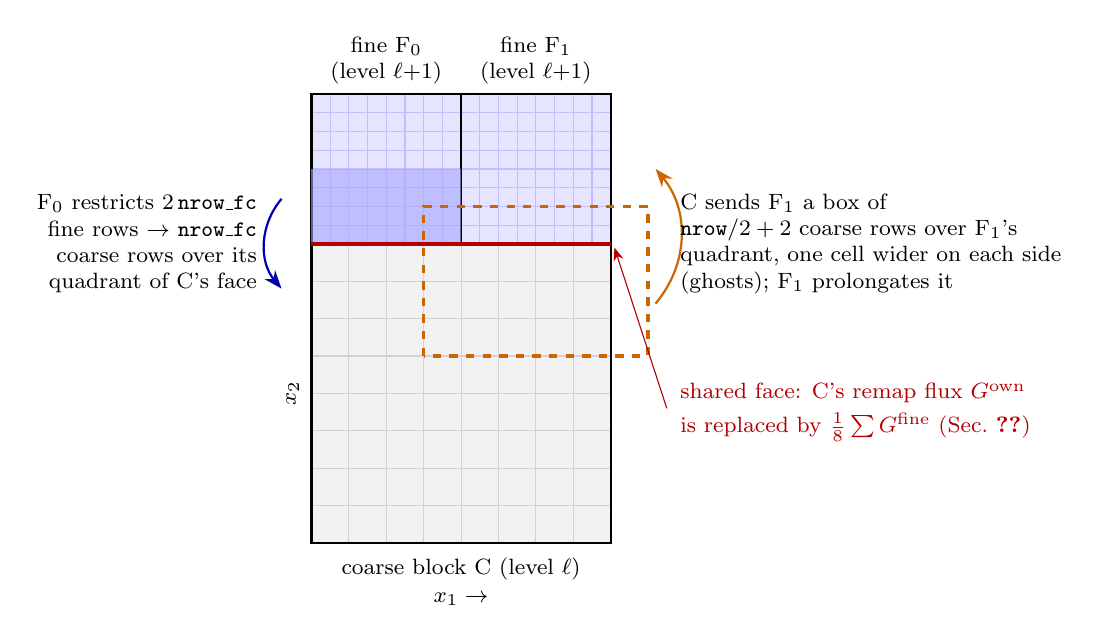
\begin{tikzpicture}[scale=0.95, every node/.style={font=\footnotesize}]
  % coarse block below, two fine blocks above (x1-x2 plane; the x3 pair is behind)
  \fill[gray!10] (0,0) rectangle (4,4);
  \foreach \x in {0.5,1,...,3.5} \draw[gray!35] (\x,0) -- (\x,4);
  \foreach \y in {0.5,1,...,3.5} \draw[gray!35] (0,\y) -- (4,\y);
  \draw[thick] (0,0) rectangle (4,4);
  \node at (2,-0.35) {coarse block C (level $\ell$)};
  \fill[blue!10] (0,4) rectangle (4,6);
  \foreach \x in {0.25,0.5,...,3.75} \draw[blue!25] (\x,4) -- (\x,6);
  \foreach \y in {4.25,4.5,...,5.75} \draw[blue!25] (0,\y) -- (4,\y);
  \draw[thick] (0,4) rectangle (2,6);
  \draw[thick] (2,4) rectangle (4,6);
  \node[align=center] at (1,6.45) {fine F$_0$\\(level $\ell{+}1$)};
  \node[align=center] at (3,6.45) {fine F$_1$\\(level $\ell{+}1$)};
  % restricted rows from F0 down to C
  \fill[blue!35, opacity=0.6] (0,4) rectangle (2,5);
  \draw[-{Stealth}, thick, blue!70!black] (-0.4,4.6) to[bend right=40] (-0.4,3.4);
  \node[align=right, anchor=east] at (-0.6,4.0) {F$_0$ restricts $2\,\code{nrow\_fc}$\\
        fine rows $\to$ \code{nrow\_fc}\\coarse rows over its\\quadrant of C's face};
  % coarse box from C to F1 (quadrant + 1 cell each side, rows across face)
  \draw[very thick, orange!80!black, dashed] (1.5,2.5) rectangle (4.5,4.5);
  \draw[-{Stealth}, thick, orange!80!black] (4.6,3.2) to[bend right=40] (4.6,5.0);
  \node[align=left, anchor=west] at (4.8,4.0) {C sends F$_1$ a box of\\
        $\code{nrow}/2+2$ coarse rows over F$_1$'s\\quadrant, one cell wider on each
        side\\(ghosts); F$_1$ prolongates it};
  % face and flux
  \draw[ultra thick, red!70!black] (0,4) -- (4,4);
  \node[red!70!black, anchor=west] at (4.8,2.0) {shared face: C's remap flux
        $G^{\rm own}$};
  \node[red!70!black, anchor=west] at (4.8,1.55) {is replaced by
        $\tfrac18\sum G^{\rm fine}$ (Sec.~\ref{sec:fluxcorr})};
  \draw[-{Stealth}, red!70!black] (4.75,1.8) -- (4.05,3.95);
  \node[rotate=90] at (-0.25,2) {$x_2$};
  \node at (2,-0.75) {$x_1 \rightarrow$};
\end{tikzpicture}
\caption{The two cross-level messages on an $x_2$ face, in the $x_1$--$x_2$ plane (the
two further fine blocks of the face are behind, in $x_3$). Each block remaps on its own
grid; the neighbor's rows arrive restricted or as a coarse box to prolongate. After the
remap, the fine blocks send their face fluxes to C.}
\label{fig:messages}
\end{figure}

\subsection{Buffers and messages}
Buffers are flat arrays per (MeshBlock, face): \code{sbuf\_oa}, \code{rbuf\_oa} of shape
$(n_{\rm mb}, 2, \code{sz\_face})$. Face $f = 0$ is the inner $x_2$ face (neighbor slots
8--11), $f = 1$ the outer (12--15). The message for sub-face $q$ (slot $8 + 4f + q$) starts
at offset $q \cdot n_{\rm var} \cdot s$, where $s$ is the per-variable size of that
message kind; variable $v$ starts at $v\,s$, and inside a variable the cells run with $i$
fastest and rows in ascending $j$:

\begin{center}
\small
\begin{tabular}{@{}lll@{}}
\toprule
Message & Cells per variable & Rows (sender) \\
\midrule
same level & $\code{sz\_same} = n_{x3}\cdot\code{nrow}\cdot n_{x1}$ &
  $j_s \ldots j_s{+}\code{nrow}{-}1$ ($f{=}0$) or $j_e{-}\code{nrow}{+}1 \ldots j_e$ \\
fine $\to$ coarse & $\code{sz\_fc} = \tfrac{n_{x3}}2\cdot\code{nrow\_fc}\cdot\tfrac{n_{x1}}2$
  & $2\,\code{nrow\_fc}$ fine rows next to the face, restricted \\
coarse $\to$ fine & $\code{sz\_cf} = (\tfrac{n_{x3}}2{+}2)\cdot\code{nrow\_cf}\cdot
  (\tfrac{n_{x1}}2{+}2)$ & $j_s{-}1 \ldots j_s{+}\code{nrow}/2$ or
  $j_e{-}\code{nrow}/2 \ldots j_e{+}1$ \\
\bottomrule
\end{tabular}
\end{center}

\noindent
with $\code{nrow\_fc} = \min(\code{nrow}, n_{x2}/2)$ and
$\code{nrow\_cf} = \code{nrow}/2 + 2$, and
\[
  \code{sz\_face} = n_{\rm var}\max\left(\code{sz\_same},\;
  4\max(\code{sz\_fc},\code{sz\_cf})\right).
\]
The coarse box of quadrant $(f_x, f_z)$ spans
$i = i_s + f_x n_{x1}/2 - 1 \ldots i_s + (f_x{+}1) n_{x1}/2$ and the same in $k$. Its
outermost cells (the row across the face and the transverse layer at the block edge) are
ghost cells.

A message lands in the receiver's buffer at the receiver's sub-face offset, read from
\code{nghbr.dest}. Senders on the same rank write straight into the receiver's buffer;
otherwise the message goes through \code{sbuf\_oa} and \code{MPI\_Isend} with tag
$(\code{dest} \ll \code{NUM\_BITS\_LID}) \,|\, \code{lid}$ on \code{comm\_orb\_advect}, as
the other boundary exchanges do. Receives are posted per sub-face in
\fn{OrbitalAdvectionCC::InitRecv}, with the size of the kind seen from the receiver; MPI
requests are kept per (block, sub-face), $8 n_{\rm mb}$ of each.

\subsection{Unpacking: index maps}
The extended column has $n_{x2} + 2\,\code{nrow}$ cells; the block's own cells start at
$j_f = \code{nrow}$. The $\code{nrow}$ rows beyond face $f$ are numbered
$t = 0 \ldots \code{nrow}-1$ in ascending $j$ (so on the inner face $t = \code{nrow}-1$
touches the block, on the outer face $t = 0$ does). Row $t$ is loaded by:
\begin{itemize}\itemsep2pt
\item \textbf{same level:} the received row $t$.
\item \textbf{finer:} quadrant $f_x = \lfloor (i-i_s)/(n_{x1}/2)\rfloor$, $f_z$ likewise;
      coarse row $t_c = t - (\code{nrow}-\code{nrow\_fc})$ on the inner face, $t_c = t$ on
      the outer. Rows with $t_c$ outside $[0, \code{nrow\_fc})$ are never read (guarded,
      Sec.~\ref{sec:shiftlimit}).
\item \textbf{coarser:} with the distance $d$ from the face ($d = \code{nrow}-1-t$ on the
      inner face, $d = t$ on the outer), the coarse cell is at box row
      $jj = \code{nrow}/2 - \lfloor d/2\rfloor$ (inner) or $\lfloor d/2\rfloor + 1$ (outer),
      box column $ii = \lfloor (i-i_s)/2\rfloor + 1$, box layer $kk$ likewise. The value is
      \begin{equation}
        c + s_1\,\delta_1 + s_2\,\delta_2 + s_3\,\delta_3, \qquad
        \delta_n = \tfrac18\left[\operatorname{sgn}(\Delta^-_n) +
        \operatorname{sgn}(\Delta^+_n)\right]\min(|\Delta^-_n|, |\Delta^+_n|),
      \end{equation}
      the \fn{ProlongCC} formula ($\Delta^\pm_n$ the one-sided differences of the coarse
      box in direction $n$), with $s_1 = -1$ for even $i - i_s$ and $+1$ for odd, $s_3$
      likewise in $k$, and $s_2 = +1$ for the fine row in the upper half of the coarse cell
      ($d$ even on the inner face, odd on the outer).
\end{itemize}

\noindent
The ghost cells used for the slopes hold the state of the previous stage's exchange:
for RK2 they differ from the updated state by $O(\Delta t^2)$, and they only enter
minmod-limited slopes. The remap shifts the coarse-box values like any other, and their
mean over each coarse cell is the coarse value, so the prolongation conserves.

%=========================================================================================
\section{The orbital-advection flux correction}
\label{sec:fluxcorr}

\subsection{The remap in flux form}
Eq.~\eqref{eq:remap} telescopes: with
\begin{equation}
  G_{j-1/2} = \begin{cases}
     \displaystyle F_{j-J-1/2} + \sum_{l=j-J}^{j-1} a_l, & J \ge 0,\\[1.2em]
     \displaystyle F_{j-J-1/2} - \sum_{l=j}^{j-J-1} a_l, & J < 0,
  \end{cases}
  \qquad
  a^{\rm new}_j = a_j - \left(G_{j+1/2} - G_{j-1/2}\right),
  \label{eq:G}
\end{equation}
$G_{j-1/2}$ is the total amount (per cell volume) moved in $+x_2$ through face
$j - 1/2$: the $|J|$ whole cells it passes plus the fractional flux. In the unpack kernel,
after the fractional fluxes are known, one thread per column evaluates $G$ at the block's
two $x_2$ faces and stores it in \code{gflx}$(m, f, v, k, i)$ (multilevel meshes only).

\subsection{Why the two sides disagree, and the correction}
Across a level jump the coarse block remaps restricted fine data with its column
velocity, and each fine block remaps prolongated coarse data with its own. Both
approximate the same transport, but not identically, so without correction the mass
that leaves one side is not the mass that enters the other (the mass drift is
$10^{-7}$--$10^{-6}$ in the tests). The fine side is taken as the better estimate, as in
the hydro flux correction. A coarse column covers $2\times2$ fine columns and the volume
ratio is $1/8$, so the amount through the coarse face is
\begin{equation}
  G^{\rm fine} = \tfrac18 \sum_{2\times2} G_f .
\end{equation}
\fn{SendFluxCC} (task \fn{SendFlx\_OA}, after \fn{RecvU\_OA}) computes this on every
block whose $x_2$ neighbor is coarser and sends it ($\tfrac{n_{x3}}2\cdot\tfrac{n_{x1}}2$
values per variable; separate communicator \code{comm\_orb\_flx}).
\fn{RecvAndCorrectFluxCC} (task \fn{RecvFlx\_OA}) replaces the coarse block's own flux
in the row next to the face:
\begin{equation}
  a_{j_s} \mathrel{+}= G^{\rm fine} - G^{\rm own} \quad\text{(inner face)}, \qquad
  a_{j_e} \mathrel{+}= G^{\rm own} - G^{\rm fine} \quad\text{(outer face)}.
\end{equation}
The two faces are separate kernels. The receives are posted with the data receives in
\fn{InitRecv}, waited for in \fn{ClearRecv}. \code{<shearing\_box> oa\_flux\_correct =
false} switches the correction off (for tests). The dust module builds its own copy of
the hydro task tail (\file{dust\_tasks.cpp}); the two tasks are inserted there too, or
the posted flux receives would never be matched.

%=========================================================================================
\section{How far the shift may reach}
\label{sec:shiftlimit}

\subsection{Rows available, and the guard}
The PPM reconstruction of the upwind cell reads two cells on either side of it, so the
remap of a block with integer shift $J$ reads $|J| + 3$ rows from its upstream neighbor
(and $\max(0, 3-|J|)$ from the other). All of them must come from the immediate $x_2$
neighbor. \fn{RowsAvailable}$(m)$ returns
\begin{equation}
  n_{\rm avail} = \begin{cases}
    \code{nrow} & \text{neither $x_2$ neighbor finer},\\
    \min(\code{nrow}, n_{x2}/2) & \text{a finer $x_2$ neighbor (a fine block is
    $n_{x2}/2$ coarse rows).}
  \end{cases}
\end{equation}
\code{nrow} defaults to $\min(n_{x2}, \code{maxjshift} + 3)$ (rounded up to even on
multilevel meshes, so that it is a whole number of coarse rows) and can be set with
\code{<shearing\_box> oa\_nrow} ($\le n_{x2}$). \fn{RecvAndUnpackCC} checks every step,
with this step's $\Delta t$ and each block's $\max|x_1|$, that
$\lfloor \qom\Delta t\max|x_1|/\Delta x_2\rfloor + 3 \le n_{\rm avail}$, and aborts
naming the block otherwise.

\subsection{The timestep limit}
\label{sec:oadt}
The guard alone would end a long AMR run the first time the mesh put a fine block next to
a coarse one at large $|x_1|$. \fn{OrbitalAdvectionCC::MaxTimeStep} therefore returns
\begin{equation}
  \Delta t_{\rm OA} = \min_m\; 0.999\,
  \frac{(n_{{\rm avail},m} - 2)\,\Delta x_{2,m}}{\qom \max|x_1|_m},
\end{equation}
which \fn{Mesh::NewTimeStep} takes into the cycle timestep (not multiplied by the CFL
number), for hydro and MHD alike. The driver calls \fn{Mesh::NewTimeStep} after the AMR
update, so the limit is evaluated on the mesh the next step will use. It binds only when
shifts are large. On $8^3$ blocks a coarse block next to a finer $x_2$ neighbor allows one
coarse cell per step: at $|x| = 32H$ and $4$ cells per $H$ on the coarse side,
$\Delta t \le 0.0104/\Om$ at the root level and $2^{-\ell}$ times that at level $\ell$. In
the SC14 runs the hydro timestep is well below this at the root level; on refined levels
the two can be comparable.

\subsection{The old buffer depth}
The previous code allocated and packed $\code{ng} + \code{maxjshift}$ rows per face,
with $\code{maxjshift} = \lfloor \mathrm{CFL}\,\qom\max|x_1|\rfloor + 1$, doubled on
multilevel meshes, and checked the shift against \code{maxjshift}. For the 64H SC14 box
on $8^3$ blocks that is $4 + 30 = 34$ rows, so the pack read far outside the 8-row block
(past the end of the array for the last block). The results were not affected, because
the actual shift stayed below one cell and those rows were never used. Buffers are now at
most one block deep ($\code{nrow} \le n_{x2}$), about $4\times$ smaller for $8^3$
blocks, and the guard compares the shift with what the neighbor can actually supply.

%=========================================================================================
\section{Policy and control flow}
\label{sec:policy}

\subsection{The refinement policy}
\begin{itemize}\itemsep2pt
\item \textbf{I1} (one uniform level along both shear-periodic $x_1$ faces) is unchanged.
\item \textbf{I2} (complete $x_2$ rings) is checked in
      \fn{Mesh::CheckShearingBoxRefinement} only with \code{<shearing\_box> oa\_annular =
      true}; the default is \code{false}.
\item The \textbf{ring-wise flag synchronization} in \fn{MeshRefinement::CheckForRefinement}
      runs only with \code{oa\_annular = true}. User criteria such as the
      \code{gravito\_turb} hold/buffer criterion then refine what they flag.
\item The \textbf{graded cap} and the $x_1$-boundary veto are unchanged.
\end{itemize}

\subsection{Task sequence of the last RK stage}
\begin{center}
\small
\begin{tabular}{@{}lp{10.5cm}@{}}
\toprule
Task & With orbital advection \\
\midrule
\fn{RKUpdate}, \fn{HydroSrcTerms} & as before \\
\fn{SendU\_OA} & \fn{PackAndSendCC}: same / restricted / coarse-box messages \\
\fn{RecvU\_OA} & \fn{RecvAndUnpackCC}: wait, guard, load + prolongate, remap, store $G$ \\
\fn{SendFlx\_OA} & \fn{SendFluxCC}: restricted $G$ to coarser $x_2$ neighbors \\
\fn{RecvFlx\_OA} & \fn{RecvAndCorrectFluxCC}: replace the face flux on coarse blocks \\
\fn{RestrictU}, \fn{SendU}, \ldots & as before \\
\bottomrule
\end{tabular}
\end{center}
\noindent
The MHD task list calls the same \fn{OrbitalAdvectionCC} for the cell-centered variables,
with the same two flux tasks, and adds two for the face fields (\S\ref{sec:mhd}).

\subsection{A test criterion: the moving box}
The shwave problem generator's prescribed moving-ring criterion (\fn{MovingRingRefine})
takes an optional $x_2$ window, $y_c(t) = y_{c0} + A_y\sin(\omega_y t) + v_y t$, wrapped
periodically into $[x_{2,\min}, x_{2,\max})$. With \code{ring\_yhwidth} $> 0$ a block is
refined only if it overlaps both the $x_1$ interval and the $x_2$ window (or one of its
periodic images): a box that moves in $x_1$ and drifts through $x_2$.

\subsection{A physical criterion: the Jeans length}
\label{sec:jeanscrit}
For the nonlinear swing (validation document, section ``Nonlinear swing to collapse'') the swing problem
generator has a Jeans-length criterion, \fn{SwingJeansRefine}, switched on by
\code{<problem> amr\_njeans} $> 0$ with \code{<amr\_criterion1> method = user}. For each
MeshBlock it takes the minimum of $c_s^2/\rho$ over the cells (with \code{amr\_buffer},
the default, over the ghost cells too, so refinement reaches a little beyond the gas that
triggered it) and forms
\[
  n_J = \frac{\lambda_J}{\Delta x_1}, \qquad
  \lambda_J = 2\pi\left(\frac{c_s^2}{4\pi G\rho}\right)^{1/2},
\]
with $c_s$ the isothermal sound speed, or $(\gamma P/\rho)^{1/2}$ for an ideal gas. The block
is flagged for refinement when $n_J < $ \code{amr\_njeans} and for derefinement when
$n_J > $ \code{amr\_njeans}$\,\times\,$\code{amr\_njeans\_deref} (default 2.5) and no other
criterion has flagged it. This is the thermal Jeans length: magnetic support is not
counted, so for MHD the criterion is conservative. It is a team reduction per block (one
kernel), on the GPU as on the CPU, and with orbital advection it needs no $x_2$
synchronization: the refined region may be any set of blocks.

%=========================================================================================
\section{Magnetic fields: MHD}
\label{sec:mhd}
This was done in two steps: first refinement in complete $x_2$ rings (the first five subsections),
then $x_2$ level jumps (\S\ref{sec:mhdB}).

\subsection{How the face-field remap works}
\fn{OrbitalAdvectionFC} (\file{orbital\_advection\_fc.cpp}) shifts the face-centred field
with constrained transport (CT) instead of remapping it directly. For each $x_2$ column of
$B_3$ (at $x_1$ cell centres) and of $B_1$ (at $x_1$ faces) it builds the extended column
from the $x_2$ neighbours, computes the remap flux exactly as for a cell-centred variable,
and turns it into an effective EMF on the $x_2$ faces, in units of $\Delta x_2$:
\begin{equation}
  \mathcal E_1 = -\left(F + \textstyle\sum_{\rm whole\ cells} B_3\right), \qquad
  \mathcal E_3 = +\left(F + \textstyle\sum_{\rm whole\ cells} B_1\right),
\end{equation}
(\code{emfx} on $x_1$ edges, \code{emfz} on $x_3$ edges; the remap has no $\mathcal E_2$).
The field is then updated by the discrete curl,
\begin{equation}
  B_1 \mathrel{-}= \delta_2 \mathcal E_3, \qquad
  B_2 \mathrel{+}= \tfrac{\Delta x_2}{\Delta x_1}\delta_1 \mathcal E_3
                 - \tfrac{\Delta x_2}{\Delta x_3}\delta_3 \mathcal E_1, \qquad
  B_3 \mathrel{+}= \delta_2 \mathcal E_1,
\end{equation}
which keeps $\nabla\!\cdot\!B$ unchanged inside every block.

\subsection{What goes wrong at a level jump, even with rings}
With rings every $x_2$ neighbour is at the block's level, so the extended columns are the
uniform ones; but the blocks still meet coarser or finer blocks across $x_1$ and $x_3$ faces.
AthenaK keeps both copies of a face shared by two blocks: the regular exchange never
overwrites a block's own boundary face (\file{buffs\_fc.cpp}: same-level and finer data
start one face beyond it). The copies stay equal only because the stage EMFs on the shared
edges are made identical (\fn{RecvAndUnpackFluxFC}: averaged between same-level blocks,
replaced by restricted fine values on coarse blocks). The remap's EMFs had no such step. A
fine block remaps its fine $B_1$ on a shared $x_1$ face, the coarse block remaps its coarse
$B_1$ on the same face, and the two results differ at truncation level: each block stays
divergence-free, but the coarse copy drifts away from the mean of the fine copies
($\sim1\%$ of the field in the tests). That was the unanalysed $\nabla\!\cdot\!B$ question
behind the old fatal error.

\subsection{The correction}
With mesh refinement \fn{RecvAndUnpackFC} no longer updates $B$. It stores the EMFs as
$E\,\Delta t$ on the edges (\code{eoa}: $\mathcal E_1\Delta x_2$ in \code{x1e},
$\mathcal E_3\Delta x_2$ in \code{x3e}, zero \code{x2e}) and returns. Two new MHD tasks
follow \fn{RecvB\_OA}:
\begin{itemize}\itemsep2pt
\item \fn{SendE\_OA} $\to$ \fn{SendEMF\_OA}: \fn{PackAndSendFluxFC} on \code{eoa};
\item \fn{RecvE\_OA} $\to$ \fn{RecvEMFAndUpdateB\_OA}: \fn{RecvAndUnpackFluxFC} on
      \code{eoa}, conversion back to units of $\Delta x_2$, and the CT update
      (\fn{UpdateB}).
\end{itemize}
The exchange is the stage's own EMF machinery, run on a private
\fn{MeshBoundaryValuesFC} instance (\code{pbval\_oa}, with its own buffers and MPI
communicators), so it cannot collide with the stage's EMF messages, whose sends are still
in flight. It handles faces and edges, same-rank copies and MPI, and skips the
shear-periodic $x_1$ boundary as the stage correction does. Physical units are needed
because the correction averages EMFs along edges: a coarse edge carries the mean of its two
fine edges, which in units of the block's own $\Delta x_2$ would carry a factor $1/2$.
Receives are posted in \fn{OrbitalAdvectionFC::InitRecv} and cleared with the base
buffers. Without refinement nothing of this runs, and the arithmetic is the old one.

\noindent
Two further changes in the class:
\begin{itemize}\itemsep2pt
\item \textbf{Buffer depth.} $B_1$, $B_3$ rows sent across an $x_2$ face:
      $\code{nrowb} = \min(n_{x2},\ \max(\code{ng} + \code{maxjshift} + 1,\
      \code{oa\_nrow}))$, at least the cell-centred \code{nrow} and never more than one
      block (the old depth $\code{ng} + \code{maxjshift}$ could exceed the block).
\item \textbf{EMF arrays} \code{emfx}, \code{emfz} are sized for the largest pack AMR
      can produce (the larger of the pack size and \code{nmb\_maxperrank}), as the other
      MHD arrays are;
      they were sized for the initial pack, which was harmless only while refinement was
      fatal.
\end{itemize}

\subsection{Policy}
In the first step \fn{MHD::MHD} accepted orbital advection on a refined mesh only with
\code{<shearing\_box> oa\_annular = true}. Since the second step (\S\ref{sec:mhdB}) the
policy is that of hydro: \code{oa\_annular} is optional. The cell-centred flux tasks
(\fn{SendFlx\_OA}, \fn{RecvFlx\_OA}) are in the MHD task list too.

\subsection{A diagnostic: shared-face consistency}
The swing problem generator's history has two more columns with MHD. After the boundary
exchange a fine block holds, in \code{coarse\_b0}, the coarse neighbour's copy of every face
they share; \code{bmis} $= \sum |B_n^{\rm coarse} - \langle B_n^{\rm fine}\rangle_{2\times2}|
\,\Delta A$ over the six faces of every fine block with a coarser neighbour, and
\code{bnrm} $= \sum |B_n|\,\Delta A$ over the same faces. Their ratio is round-off when the
copies agree.

\subsection{Across \texorpdfstring{$x_2$}{x2} level jumps}
\label{sec:mhdB}
The face-field remap reads $B_3$ (on $x_3$ faces) and $B_1$ (on $x_1$ faces) beyond the
block's $x_2$ faces. The exchange now mirrors the cell-centred one
(\S\ref{sec:design}): flat buffers per (MeshBlock, face) (\code{sbufb}, \code{rbufb}),
sub-face $q$ at $q\cdot 2\,s$, component $c$ ($0$: $B_3$, $1$: $B_1$) at $c\,s$, one
footprint $(n_{x3}{+}1)\times\text{rows}\times(n_{x1}{+}1)$ for both components (the unused
$B_3$ at $i_e{+}1$ and $B_1$ at $k_e{+}1$ are carried along), MPI requests per sub-face.

\begin{center}
\small
\begin{tabular}{@{}lp{11cm}@{}}
\toprule
Neighbour & Rows the receiver gets \\
\midrule
same level & \code{nrowb} rows of $B_3$, $B_1$, copied \\
finer      & per quadrant, $\code{nrowb\_fc} = \min(\code{nrowb}, n_{x2}/2)$ coarse rows:
             each coarse face value the mean of the $2\times2$ fine faces it covers
             (area average; $B_3$ over $x_1, x_2$, $B_1$ over $x_2, x_3$) \\
coarser    & a coarse box over the block's quadrant, one extra layer on every side,
             $\code{nrowb}/2 + 2$ rows; interpolated by the receiver \\
\bottomrule
\end{tabular}
\end{center}

\noindent
The interpolation from the coarse box treats each component on its own lattice. Along the
component's normal direction a fine face either coincides with a coarse face (value taken
there) or lies midway between two (mean of the two). In the two transverse directions the
minmod-limited slopes of \fn{ProlongCC} move the value to the fine position ($\pm\frac14$
of a coarse cell, with the $\frac18[\operatorname{sgn}+\operatorname{sgn}]\min$ form).
This is not the divergence-preserving prolongation of AthenaK's ghost zones, and need not
be: the buffer rows only feed the remap's EMFs, and CT keeps $\nabla\!\cdot\!B$ unchanged for
any EMFs. A face on a quadrant boundary of a coarse receiver is read from the upper
quadrant (both fine copies are equal).

The EMFs on the $x_2$ faces and edges at level jumps are corrected by the same private
\fn{MeshBoundaryValuesFC} instance as those on $x_1$, $x_3$ faces: it handles every face
and edge neighbour, so nothing was added there. \code{nrowb} is rounded up to even on
multilevel meshes and is at least the cell-centred \code{nrow}, so the cell-centred
timestep limit and guard (\S\ref{sec:shiftlimit}) cover the face fields too. The same-level
path is unchanged: uniform runs and the ring runs of the first step are bit-identical.

The swing problem generator's moving-ring criterion takes the same optional $x_2$ window
as the shwave one (\code{ring\_yc0}, \code{ring\_yamp}, \code{ring\_yfreq},
\code{ring\_yvel}, \code{ring\_yhwidth}).

%=========================================================================================
\section{Input-file interface}
\label{sec:inputs}

\subsection{Parameters}
\begin{center}
\small
\begin{tabular}{@{}>{\raggedright\arraybackslash}p{2.6cm}>{\raggedright\arraybackslash}p{3.4cm}>{\raggedright\arraybackslash}p{2.6cm}p{5.4cm}@{}}
\toprule
Block & Parameter & Default & Meaning \\
\midrule
\code{<shearing\_box>} & \code{oa\_annular} & \code{false} & \code{true}: complete $x_2$
  rings required (I2) and AMR flags synchronized ring-wise \\
 & \code{oa\_flux\_correct} & \code{true} & Orbital-advection flux correction at $x_2$
  level jumps (\code{false} for tests only) \\
 & \code{oa\_nrow} & $\min(n_{x2},$ \code{maxjshift}$\,{+}\,3)$ & Rows sent across a same-level
  $x_2$ face; at most $n_{x2}$ \\
\midrule
\code{<problem>} (shwave) & \code{ring\_yc0}, \code{ring\_yamp} & 0 & Window center and
  oscillation amplitude \\
 & \code{ring\_yfreq}, \code{ring\_yvel} & 1, 0 & Oscillation frequency and drift speed \\
 & \code{ring\_yhwidth} & $-1$ & $> 0$: refine only inside the $x_2$ window \\
\code{<problem>} (swing) & \code{amr\_njeans} & $-1$ & $> 0$: Jeans criterion,
  refine where $\lambda_J <$ this many cells (\S\ref{sec:jeanscrit}) \\
 & \code{amr\_njeans\_deref} & 2.5 & derefine where $\lambda_J$ exceeds
  \code{amr\_njeans} times this everywhere in the block \\
 & \code{amr\_buffer} & \code{true} & include the ghost cells \\
\bottomrule
\end{tabular}
\end{center}
\noindent
Command-line overrides replace only parameters already in the input file, so
\code{oa\_annular} and \code{oa\_flux\_correct} must be written into a copy of the input
when they are to be changed and are not there.

\subsection{Reference inputs}
\begin{center}
\small
\begin{tabular}{@{}>{\raggedright\arraybackslash}p{8.6cm}p{5.8cm}@{}}
\toprule
File (under \file{inputs/}) & Configuration \\
\midrule
\file{shearing\_box/epicycle\_smr\_ypatch.athinput} & Epicycle, level-1 patch over
  part of $x_2$ \\
\file{shearing\_box/hydro\_incompress\_shwave\_smr\_ypatch.athinput} & Vortical shwave,
  static patch \\
\file{shearing\_box/hydro\_incompress\_shwave\_amr\_box.athinput} & Vortical shwave,
  moving box (AMR) \\
\file{tests/swing\_selfgrav\_smr\_ypatch.athinput} & Swing with multigrid gravity, patch \\
\file{tests/swing\_selfgrav\_clump\_jeans.athinput} & Nonlinear swing to collapse,
  Jeans-criterion AMR \\
\file{tests/swing\_mhd\_clump\_jeans.athinput} & The same, magnetized ($\beta = 8$) \\
\bottomrule
\end{tabular}
\end{center}

%=========================================================================================
\section{Guard reference}
\label{sec:guards}
\begin{center}
\small
\begin{tabular}{@{}>{\raggedright\arraybackslash}p{4.4cm}>{\raggedright\arraybackslash}p{4.4cm}p{5.4cm}@{}}
\toprule
Location & Condition & Protects \\
\midrule
\fn{OrbitalAdvectionCC::\-RecvAndUnpackCC} & integer shift $+\,3 >$ rows available from
  the $x_2$ neighbors & The remap stencil stays inside the immediate neighbor; normally
  prevented by the timestep limit \\
\fn{Mesh::CheckShearingBox\-Refinement} & incomplete $x_2$ ring with
  \code{oa\_annular = true} & The optional annular policy \\
\fn{Mesh::CheckShearingBox\-Refinement} & $x_1$-face blocks on more than one level & I1
  (unchanged) \\
\fn{MHD::MHD} & (removed) & MHD $+$ orbital advection $+$ refinement is allowed \\
\bottomrule
\end{tabular}
\end{center}

%=========================================================================================
\section{Limitations and next steps}
\label{sec:limits}
\begin{enumerate}\itemsep4pt
\item \textbf{$\nabla\!\cdot\!B$ at AMR derefinement next to fine $x_2$ neighbours.}
      Not part of this work, found by it: when a refined \emph{box} (bounded in $x_1$ and
      $x_2$) is partly derefined, $|\nabla\!\cdot\!B|/|B|$ jumps by $10^{-13}$--$10^{-12}$
      per event, with or without orbital advection and with $q = 0$; a moving ring does
      not. AthenaK's AMR face-field handling (likely \fn{RepairAMRFC} or the face
      ownership at $x_2$ faces and $x_1x_2$ edges) is the suspect (validation document).
\item \textbf{One neighbor deep.} All upstream data come from the immediate $x_2$
      neighbor; the timestep limit enforces it. Reaching through two neighbors would lift
      the limit on small blocks far from $x = 0$.
\item \textbf{Previous-stage ghosts in the coarse box.} They enter only the limited
      slopes of the prolongation; a separate orbital-advection stage with its own
      boundary cycle (as in Athena++) would remove this at the cost of an extra exchange.
\item \textbf{Non-FARGO refinement with $x_2$ level jumps} collapses at the first step
      ($\Delta t \to 10^{-45}$) --- in the parent code too, with or without
      \code{prolong\_primitives}. It is outside this work.
\item \textbf{Production test pending.} The SC14 clump-following AMR with and without
      rings (block count and cost) has not been run yet.
\end{enumerate}

\end{document}
